\documentclass[11pt,a4paper]{article}

\usepackage[utf8]{inputenc} 
\usepackage[T1]{fontenc} 
\usepackage{lmodern}
\usepackage[margin=2cm]{geometry}
\usepackage[german]{babel}
\usepackage{amsmath} 
\usepackage{graphicx} 
\usepackage{cancel}
\usepackage{booktabs}
\usepackage{hyperref}
\usepackage{tikz}
\hypersetup{
    colorlinks,
    citecolor=red,
    filecolor=black,
    linkcolor=black!20!blue!90!,
    urlcolor=black} 
\usepackage{nicefrac}
%\usepackage[table]{xcolor}
\usepackage{tocloft}

\setlength{\parindent}{0pt}
\setlength{\parskip}{1ex plus 0.5ex minus 0.5ex}

\definecolor{incolor}{rgb}{0.0, 0.0, 0.5}

\hbadness=99999

\newcommand{\refpy}[1]{Siehe Anhang: \textit{Rechnungen in Python} (\texttt{{\color{incolor}In [{\color{incolor}#1}]}})}
\newcommand\dif{\mathop{}\!\mathrm{d}}
\newcommand{\halftime}[4]{\begin{figure}[h]
\begin{minipage}{.#1\textwidth}#3\end{minipage}\begin{minipage}{.#2\textwidth}
\centering
#4\end{minipage}
\end{figure}}
\renewcommand{\vec}{\boldsymbol}
\newcommand\mean{\begin{equation}
\bar{x}=\frac{\sum_{i=1}^n x_{i}}{n}\label{mean}
\end{equation}}
\newcommand\meanstd{\begin{equation}
s_{\bar{x}}=\frac{s_x}{\sqrt{n}}\label{meanstd}
\end{equation}}
\newcommand\prodquo{\begin{equation}\left\vert\frac{\Delta z}{z}\right\vert=\sqrt{\left(a\frac{\Delta x}{x}\right)^2+\left(b\frac{\Delta y}{y}\right)^2+\ldots}\textrm{ f\"ur }z=x^a\ y^b\ldots\end{equation}}
\newcommand\tfunc{\begin{equation}
\frac{\vert x-y_0\vert}{u_x}
\end{equation}}

\begin{document}
{
\centering 
\large 
Physiklabor für Anf\"anger*innen \\
Ferienpraktikum im Sommersemester 2018 \\[4mm]
\textbf{\LARGE 
Versuch 70: Linsen und Linsensysteme
} \\[3mm]
(durchgef\"uhrt am 28.09.2018 bei Daniel Bartel) \\
Andréz Gockel, Patrick M\"unnich\\
\today \\[10mm]
}

\vspace{50pt}
\tableofcontents
\pagebreak

\section{Ziel des Versuchs}

Das Ziel dieses Versuchs ist es, Einzellinsen und Linsenkombinationen zu untersuchen. Genauer schaut man, wann mit welchen Linsen scharfe Abbildungen von Gegenst\"anden vorhanden sind.

\section{Aufbau}

\halftime{5}{5}{Vorhanden sind: eine optische Bank, verschiedene Linsen (80\,mm, 150\,mm, $-200$\,mm und 250\,mm), ein Schirm, eine LED und ein Dia, alle mit jeweils eigenem Halterungsger\"at. F\"ur den letzten Teil sind auch noch rote und blaue Farbfilter, welche in die Halterung f\"ur das Dia passen, sowie auch ein Spiegel mit Halterung vorhanden.}{\fbox{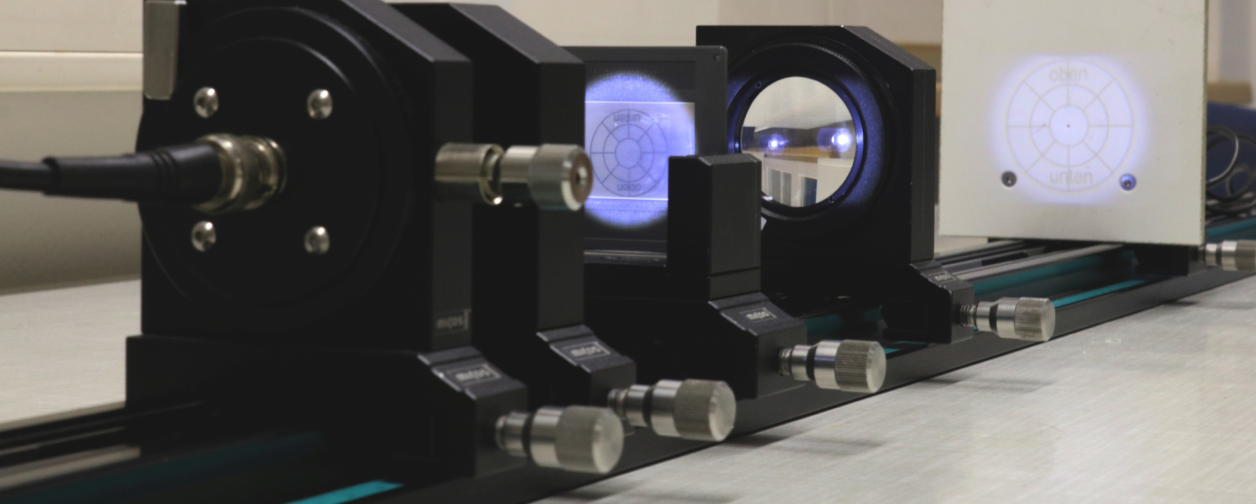
\includegraphics[width=0.5\textwidth]{aufbau.png}}
   \renewcommand\thefigure{BX}
\caption{Versuchsaufbau Teil 1 \cite{Anleitung}}
\label{Pic:1}}

\section{Teil 1: Abbildungen mit Einzellinsen und Linsensystemen}

\subsection{Theorie}

F\"ur das Verst\"andnis dieses Teils ben\"otigt man die Abbildungsgleichung f\"ur d\"unne Linsen,
\begin{equation}
\frac{1}{f}=\frac{1}{g}+\frac{1}{b},\label{eq:1}
\end{equation}

und die entsprechende Gleichung f\"ur Linsensysteme mit zwei Linsen,
\begin{equation}
\frac{1}{f}=\frac{1}{f_1}+\frac{1}{f_2}-\frac{d}{f_1f_2}.\label{eq:2}
\end{equation}

Dieses l\"asst sich f\"ur kleine Abst\"ande $d$ zwischen den Linsen zu
\[
\frac{1}{f}\approx\frac{1}{f_1}+\frac{1}{f_2}
\]
vereinfachen.


\subsection{Durchführung}

Eine Sammellinsen das Objekt, die LED und der Schirm werden auf die optische Bank gesetzt. Reihenfolge ist LED, Dia, Linse und dann Schirm.
Um die Messwerte zu bestimmen wird zuerst der Schirm in eine Position gebracht, dann die Linse bewegt, bis ein scharfes Bild entsteht. Dies wird mehrmals f\"ur verschiedene Positionen des Schirms und verschiedenen Linsensystemen (80\,mm und nichts, 80\,mm und 150\,mm und 80\,mm und $-200$\,mm) durchgef\"uhrt. Bei jeder Messreihe sollen sowohl Maxima und Minima bestimmt werden, also wann eine gro\ss e Abbildung am gr\"o\ss ten ist und wann die entsprechende kleine Abbildung am gr\"o\ss ten ist.

\subsection{Auswertung}

In diesem Teil wollen wir einfach $\nicefrac{1}{b}$ gegen $\nicefrac{1}{g}$ auftragen. Die gesch\"atzten Fehler werden als Fehlerbalken eingezeichnet. Zum Vergleich werden noch Geraden addiert, welche f\"ur die Linse mit $f=80\,$mm mit
\[
\frac{1}{b}=\frac{g}{f}
\]
berechnet wurde und f\"ur die Linsensysteme mit jeweils $f_1=80\,$mm und $f_2=150\,$mm bzw. $f_1=80\,$mm und $f_2=200\,$mm mit
\[
\frac{1}{f_1}+\frac{1}{f_2}-\frac{1}{g}
\]
bestimmt. Die resultierende Graphik mit Fehlerbalken kann im Anhang als Abbildung \ref{Abb:1} gefunden werden.

\subsection{Diskussion}

Betrachten wir unsere Graphik, so k\"onnen wir starke Abweichungen zwischen den Positionen der Geraden und denen der Verkn\"upfungsverl\"aufe der Messwerte erkennen. Jedoch verlaufen die Messpunkte klar linear und haben auch sehr \"ahnliche Steigungen wie die theoretischen Werte. 

Daraus schlie\ss en wir, dass die theoretischen \"Uberlegungen durchaus sinnvoll sein sollten. Die Abweichungen der Positionen selbst liegt wohl aufgrund von Fehlern entweder beim Messen von $g$ oder aufgrund von nicht vollst"andig korrekten Angaben bei den Linsen.

Verbesserungen k"onnten hier nur durch erleichterte Messung der genauen Position der Objekte stattfinden. Hierzu k"onnte man bspw. genau unter den Positionen Schlitze machen, wodurch man die genaue Position sehen kann.

\section{Teil 2: Bessel-Verfahren: Bestimmung der Brennweite ohne Hauptebenen}

\subsection{Theorie}

F\"ur diesen Teil f\"uhren wir neue Variablen ein:
\begin{itemize}
\item Abstand $s=g+b$ zwischen Gegenstand und Bild
\item Differenz $e=|g-b|$ zwischen den Linsenpositionen.
\end{itemize}

Diese Variablen setzen wir in (\ref{eq:1}) ein und erhalten:

\[
\frac{1}{f}=\frac{2}{s+e}+\frac{2}{s-e}
\]
\[
=\frac{2s-\bcancel{2e}+2s+\bcancel{2e}}{s^2-e^2}
\]
\[=\frac{4s}{s^2-e^2}\]
\begin{equation}
f=\frac{s^2-e^2}{4s}\label{eq:3}
\end{equation}

\subsection{Durchführung}

Wir k\"onnen in diesem Teil den selben Versuchsaufbau und die selben Messwerte wie f\"ur den ersten Teil verwenden.

\subsection{Auswertung}

In diesem Teil wollen wir einfach mit unseren Messwerten und der Formel (\ref{eq:3}) zuerst unsere Werte f\"ur $(s,e)$:



Wir k\"onnen hier die Rechnungen per Hand mit Gau\ss scher Fehlerfortpflanzung durchf\"uhren. Hierzu m\"ussen wir unsere Gleichung einfach nach jeweils $e$ und $s$ partiell ableiten:

\[
\frac{\partial f}{\partial s}=\frac{s^2+e^2}{4s}
\]
\[
\frac{\partial f}{\partial e}=\frac{-e}{2s}
\]

Dies k\"onnen wir in
\[
\Delta f=\sqrt{\left(\frac{\partial f}{\partial s}\Delta s\right)^2+\left(\frac{\partial f}{\partial e}\Delta e\right)^2}
\]
einsetzen und berechnen. In diesem Fall sind unsere Ergebnissen jedoch mit dem \textit{uncertainties} Paket in Python berechnet worden. \refpy{12} Dieses Paket hat die F\"ahigkeit, Korrelationen zwischen Variablen zu ber\"ucksichtigen \cite{Uncertainties}.

Da uns hier die Mittelwerte interessieren, nutzen wir noch

\mean

f\"ur die Berechnung des Mittelwerts und

\meanstd

f\"ur der Berechnung der Unsicherheit dessen.

Wir erhalten daraus f\"ur die Linse mit $f=80\,$mm $\bar{f}=(91\pm1)\,$mm, f\"ur das System mit $f_1=80\,$mm und $f_2=150\,$mm $\bar{f}=(69\pm2)\,$mm und f\"ur das Linsensystem mit $f_1=80\,$mm und $f_2=200\,$mm $\bar{f}=(131\pm1)\,$mm.

\subsection{Diskussion}

Unsere theoretischen Werte f"ur die Brennweiten k"onnen wir einfach mit (\ref{eq:2}) berechnen. 

Wir erhalten f"ur die $f=80\,$mm Linse offensichtlich $f=80$\,mm.

Zum Vergleich nutzen wir die $t$-Funktion:

\begin{equation}
t=\frac{\vert x-y_0\vert}{u_x}\label{eq:t}
\end{equation}

Wir erhalten $t=6.75$. Da dies au\ss erhalb des erw"unschten $t<2$-Bereichs liegt, impliziert dies Unvertr"aglichkeit der Werte.

F"ur das System mit $f_1=80\,$mm und $f_2=150\,$mm erhalten wir mittels (\ref{eq:2}) $f=57\,$mm und mit (\ref{eq:t}) $t=6.19$. Gleich wie zuvor impliziert dies Unvertr"aglichkeit.

F"ur das $f_1=80\,$mm und $f_2=-200\,$mm System erhalten wir mittels (\ref{eq:2}) $f=11.4\,$mm und (\ref{eq:t}) $t=12.2$. Dies impliziert auch Unvertr"aglichkeit.

Wir m"ussen also davon ausgehen, dass unsere Messreihen nicht ausreichend gut durchgef"uhrt wurden oder, dass systematische Fehler vorliegen. Diese m"ussten gleich wie beim vorherigen Teil sein.

Da beim vorherigen Teil zumindest die Steigung korrekt aussieht m"ussen wir davon ausgehen, dass entweder die Linsen schlechte Werte bedruckt hatten oder ein Rechenproblem bei diesem Aufgabenteil vorliegt. Ein derartiges Problem konnte jedoch nicht identifiziert werden.

\section{Teil 3: Abbe-Verfahren: Bestimmung von Brennweite und Hauptebenen}

\subsection{Theorie}

F\"ur das Abbe-Verfahren f\"uhren wir den Abbildungsma\ss stab ein:
\begin{equation}
\beta=\frac{B}{G}=\frac{b}{g}\label{eq:4}
\end{equation}
Dies machen wir, da wir $b$ und $g$ nicht direkt bestimmen k\"onnen, jedoch die Bildgr\"o\ss e $B$ und Gegenstandsgr\"o\ss e $G$ problemlos bestimmen k\"onnen.

Die Hauptebenen befinden sich dann um $h_{1/2}$ vor bzw. hinter diesem Punkt. Mit unserer messbaren scheinbaren Gegenstandsgr\"o\ss e $g'$ und scheinbare Bildweite $b'$ haben wir also
\begin{equation}
g'=\left(1+\nicefrac{1}{\beta}\right)f_1+h_1\label{eq:5}
\end{equation}
\begin{equation}
b'=\left(1+\beta\right)f_2+h_2\label{eq:6}
\end{equation}

\subsection{Durchführung}

Eigentlich ist die Durchf\"uhrung \"ahnlich zu denen von den vorherigen Teilen. Der Unterschied hier ist, dass f\"ur Linsensysteme von 80\,mm \& $-200$\,mm und $-200$\,mm \& 80\,mm zehn verschiedene Messreihen gemacht werden, wobei nur die Position der Linse f\"ur die gro\ss e Abbildung und die Gr\"o\ss e der gro\ss en Abbildung untersucht werden.

\pagebreak

\subsection{Auswertung}

In diesem Teil wollen wir zuerst mit den Formeln (\ref{eq:4}), (\ref{eq:5}) und (\ref{eq:6}) $g'$, $b'$, $\beta$ und $\Delta \beta$ bestimmen. Wir erhalten aus unseren Messreihen:

Um dies visuell darzustellen, tragen wir $1+\nicefrac{1}{\beta}$ gegen $g'$ und $1+\beta$ gegen $b'$ auf. Diese Graphen k"onnen im Anhang als Abbildung \ref{Abb:g} und \ref{Abb:b} gefunden werden.

Aus der linearen Regression k\"onnen wir $f_1$, $f_2$, $h_1$ und $h_2$ bestimmen. 

Zur Bestimmung der linearen Regression wenden wir folgende Formeln an:

\begin{equation}
a=\frac{n\sum x_iy_i-\sum x_i\sum y_i}{n\sum x_i^2-(\sum x_i)^2}
\end{equation}
\begin{equation}
\Delta a=s\sqrt{\frac{n}{n\sum x_i^2-(\sum x_i)^2}},
\end{equation}
\begin{equation}
b=\frac{\sum x_i^2\sum y_i-\sum x_i\sum x_iy_i}{n\sum x_i^2-(\sum x_i)^2}
\end{equation}
\begin{equation}
\Delta b=s\sqrt{\frac{\sum x_i^2}{n\sum x_i^2-(\sum x_i)^2}}
\end{equation}
\begin{equation}
s=\sqrt{\frac{1}{n-2}\sum^n_{i=1}[y_i-(a+bx_i)]^2},
\end{equation}

Die $a$ und $b$ sind jeweils $f$ und $h$ gleich.

Wir erhalten als Werte:

\begin{table}[h]
\centering
\caption{Berechnete Werte f\"ur Brennweiten und Abstand Hauptebenen von $\beta$} \vspace{11pt}
\begin{tabular}{cccc}
\toprule
\textrm{Wert} & $f_1$/\textrm{mm} & $f_2$/\textrm{mm} & \textrm{Ergebnis}/\textrm{cm} \\
\midrule 
$f_1$ & 80 & -200 & $11.0\pm0.3$\\
$h_1$ & 80 & -200 & $3.9\pm0.4$\\
$f_2$ & 80 & -200 & $11.6\pm0.1$\\
$h_2$ & 80 & -200 & $2.0\pm0.4$\\
$f_1$ & -200 & 80 & $11.5\pm0.3$\\
$h_1$ & -200 & 80 & $0.6\pm0.4$\\
$f_2$ & -200 & 80 & $11.93\pm0.06$\\
$h_2$ & -200 & 80 & $3.2\pm.0.4$\\
\bottomrule
\end{tabular}
\label{Tab:1}
\end{table}


Zur Klarifizierung fertigen wir noch eine (au\ss er der Linsen) ma\ss stabsgetreue Skizze an. Diese kann im Anhang als Abbildung \ref{Abb:2} gefunden werden.\\

\subsection{Diskussion}

Betrachten wir unsere Ma\ss stabsgetreue Skizze, so stimmen zumindest in diesem Fall unsere berechneten Wert f"ur $f$ prima "uberein. Dies deutet schonmal darauf, dass diese Werte gut sein sollten.

Schon im vorherigen Teil wurden die theoretischen Brennweiten f"ur ein Linsensystem aus Linsen mit Brennweiten von $f_1=80$\,mm und $f=-200$\,mm berechnet. Zur Erinnerung lag dieser Wert bei $f=11.4$\,mm. Vergleichen wir unsere Werte, so ist es sinnvoll, zuerst diese zu mitteln. Wir verwenden dazu wieder (\ref{mean}) und (\ref{meanstd}). Unsere Werte lauten dann:

\begin{itemize}
\item $f_1=80\,$mm und $f_2=-200\,$mm hat $\bar{f}=(11.3\pm0.2)$\,cm
\item $f_1=-200\,$mm und $f_2=80\,$mm hat $\bar{f}=(11.7\pm0.1)$\,cm
\end{itemize}

Erstmal ohne Fehler und $t$: Der erste Wert ist 99\% von dem theoretischen und der zweite 103\%. Diese Werte sind also wesentlich n"aher am erw"unschten Ergebnis als die vorher berechneten.

Nutzen wir aber (\ref{eq:t}), so erhalten wir f"ur die erste Messreihe $t=73.9$ und f"ur die zweite $t=80.2$. Dies impliziert starke Unvertr"aglichkeit der Ergebnisse mit dem theoretischen Wert. Unsere Fehler wurden also zu klein abgesch"atzt. Jedoch muss man auch damit rechnen, dass die Fehler aus den vorherigen Versuchsteilen hier auch existieren.

Da unsere $t$-Werte jedoch so viel gr"o\ss er sind w"are es vermutlich sinnvoll gewesen, gr"o\ss ere Fehler f"ur die Bildgr"o\ss e zu verwenden. Andere Fehler die in den vorherigen Teilen nicht existierten gibt es ja nicht. Zu schlechtes Abmessen und nicht perfektes Finden der besten Punkte f"ur die Sch"arfe k"onnten diese Werte stark beeinflusst haben.

In den Graphiken kann man sich noch "uberlegen, ob es Sinn machen w"urde, bei beiden Geraden die gleichen Steigungen zu erzwingen. Dies ist jedoch nicht wirklich n"otig, da die Werte schon nah genug aneinander sind.

Es gelten die gleichen Verbesserungsvorschl"age wie zuvor auch.

\section{Teil 4: Autokollimationsverfahren und Dispersion}

\subsection{Theorie}

Das Autokollimationsverfahren l\"asst einen leicht Brennweiten bestimmen. Die Idee hier ist einfach:

\begin{equation}
f=D\label{eq:7}
\end{equation}

Hier steht $D$ f\"ur den Abstand zwischen Gegenstand und Linsenmitte.

Dies gilt f\"ur den unten beschriebenen Versuchsaufbau.

Um zus\"atzlich noch den Einfluss der Brechzahl zu \"uberpr\"ufen, betrachten wir die Formel f\"ur die Brennweite bei symmetrischen d\"unnen Linsen:

\begin{equation}
f=\frac{1}{n-1}\left(\frac{R_1R_2}{R_2-R_1}\right)\label{eq:8}
\end{equation}

Dies impliziert, dass

\begin{equation}
\nicefrac{1}{f}\propto n-1.\label{eq:9}
\end{equation}

\subsection{Durchführung}

Wie schon erw\"ahnt werden hier Spiegel und Farbfilter zunutze gemacht. Zuerst nimmt man kein Farbfilter, aber setzt den Spiegel direkt hinter der Linse. Man bewegt die Linse dann so, bis das zur\"uckgespiegelte Bild maximal scharf ist, und notiert die Position dann. Dies wird f\"ur Linsensysteme mit 80\,mm, 150\,mm, 80\,mm \& 150\,mm, 80\,mm \& $-200$\,mm und $-200$\,mm \& 80\,mm durchgef\"uhrt.

F\"ur den Teil mit den Farbfiltern untersuchen wir \"ahnlicherma\ss en die Position der 250\,mm Linse, bei der das zur\"uckgespiegelte Bild maximal ist. Hierf\"ur wird unser Farbfilter hinter das Dia gestellt. Dies wird f\"ur rot, blau und wei\ss\ durchgef\"uhrt.

\pagebreak

\subsection{Auswertung}

Mit unseren Messdaten kommen wir mittels (\ref{eq:7}) und (\ref{eq:2}) auf folgende Ergebnisse:

\begin{table}[h]
\centering
\caption{Berechneten und gemessenen Brennweiten f\"ur verschiedene Linsensysteme} \vspace{11pt}
\begin{tabular}{cccc}
\toprule
\textrm{Erste Linse}/\textrm{mm} & \textrm{Zweite Linse}/\textrm{mm} & \textrm{Berechnet}/\textrm{mm} & \textrm{Gemessen}/\textrm{mm} \\
\midrule 
0 & 80 & 8.0 & 8.0 \\
0 & 150 & 15.0 & 14.9 \\
80 & 150 & 5.7 & 7.1 \\
80 & -200 & 11.4 & 14.6 \\
-200 & 80 & 11.4 & 10.7 \\
\bottomrule
\end{tabular}
$\begin{array}{l}
\textrm{Unsicherheiten:}\quad
\textrm{Gemessene Brennweite: } \pm 0.3 \textrm{mm}\\
\end{array}$
\label{Tab:X}
\end{table}

F\"ur den Vergleich der Brechzahlen bekommen wir theoretisch mittels (\ref{eq:9}) einen Unterschied von 1\%. Hier wurde gerechnet:

\[
\alpha_t=\frac{n_b}{n_r}
\]

F\"ur die gemessenen Werte rechnen wir dann

\[\alpha_c=\frac{D_r}{D_b}.\]

Wir erhalten einen Unterschied von $2\%\pm2\%$.

\subsection{Diskussion}

Zur "Uberpr"ufung der Korrektheit des ersten Satzes an Messungen k"onnen wir wieder einfach (\ref{eq:t}) anwenden. Wir erhalten

\begin{table}[h]
\centering
\caption{$t$-Werte f"ur ersten Teil des vierten Versuchsteils} \vspace{11pt}
\begin{tabular}{ccc}
\toprule
\textrm{Erste Linse}/\textrm{mm} & \textrm{Zweite Linse}/\textrm{mm} & $t$ \\
\midrule 
0 & 80 & 0.0 \\
0 & 150 & 0.3 \\
80 & 150 & 4.6 \\
80 & -200 & 10.6 \\
-200 & 80 & 2.4 \\
\bottomrule
\end{tabular}
\label{Tab:X}
\end{table}

Unsere $t$-Werte f"ur die Linsensysteme mit nur einer Linse sind also vertr"aglich, w"ahrend die anderen dies nicht sind. Es kann also sein, dass die angegebenen Werte f"ur die Distanz der Linsen nicht ganz korrekt ist. Dies w"are ein systematischer Fehler auf unser Ergebnis.

Dies impliziert, dass bei den vorherigen Messreihen eventuell schlecht abgelesen wurde oder ein allgemeiner Fehler dort vorhanden ist, welcher hier durch die Vorgehensweise eliminiert wurde.

Als Vorschlag gibt es zu diesem Teil nur, dass man eventuell noch selbst die Distanz zwischen den Linsen berechnen sollte.

F"ur den zweiten Teil ist eigentlich auch klar, dass die Werte vertr"aglich sind, da der gemessene Unterschied $\nicefrac{1}{2}\sigma$ von dem berechneten entfernt ist. Dies impliziert wieder, dass die Messung auf diese Weise besser funktioniert als die vorherige. Die Farbfilter scheinen auch gut auf die erw"unschten Wellenl"angen eingeschr"ankt zu haben. Dies ist ansonsten als systematischer Fehler zu behandeln. Vorschl"age gibt es hier keine.


\begin{thebibliography}{9}
\bibitem{Uncertainties}''Correlations between variables are automatically handled, which sets this module apart from many existing error propagation codes.'' - \url{https://pythonhosted.org/uncertainties/}
\bibitem{Anleitung} Physikalisches Institut der Albert-Ludwigs-Universität Freiburg (Hrsg.) (08/2018): Versuchsanleitungen zum Physiklabor für Anfänger*innen, Teil 1, Ferienpraktikum im Sommersemester 2018.
\end{thebibliography}

\section{Anhang: Abbildungen}% Tabellen und Diagramme}



%\begin{figure}[p]
%\centering
%\fbox{\includegraphics[width=0.8\textwidth]{NAME}}
%\renewcommand\thefigure{BX}
%\caption[XXXX]{XXXX}
%\label{Abb:X}
%\end{figure}

\begin{figure}[p]
\centering
\fbox{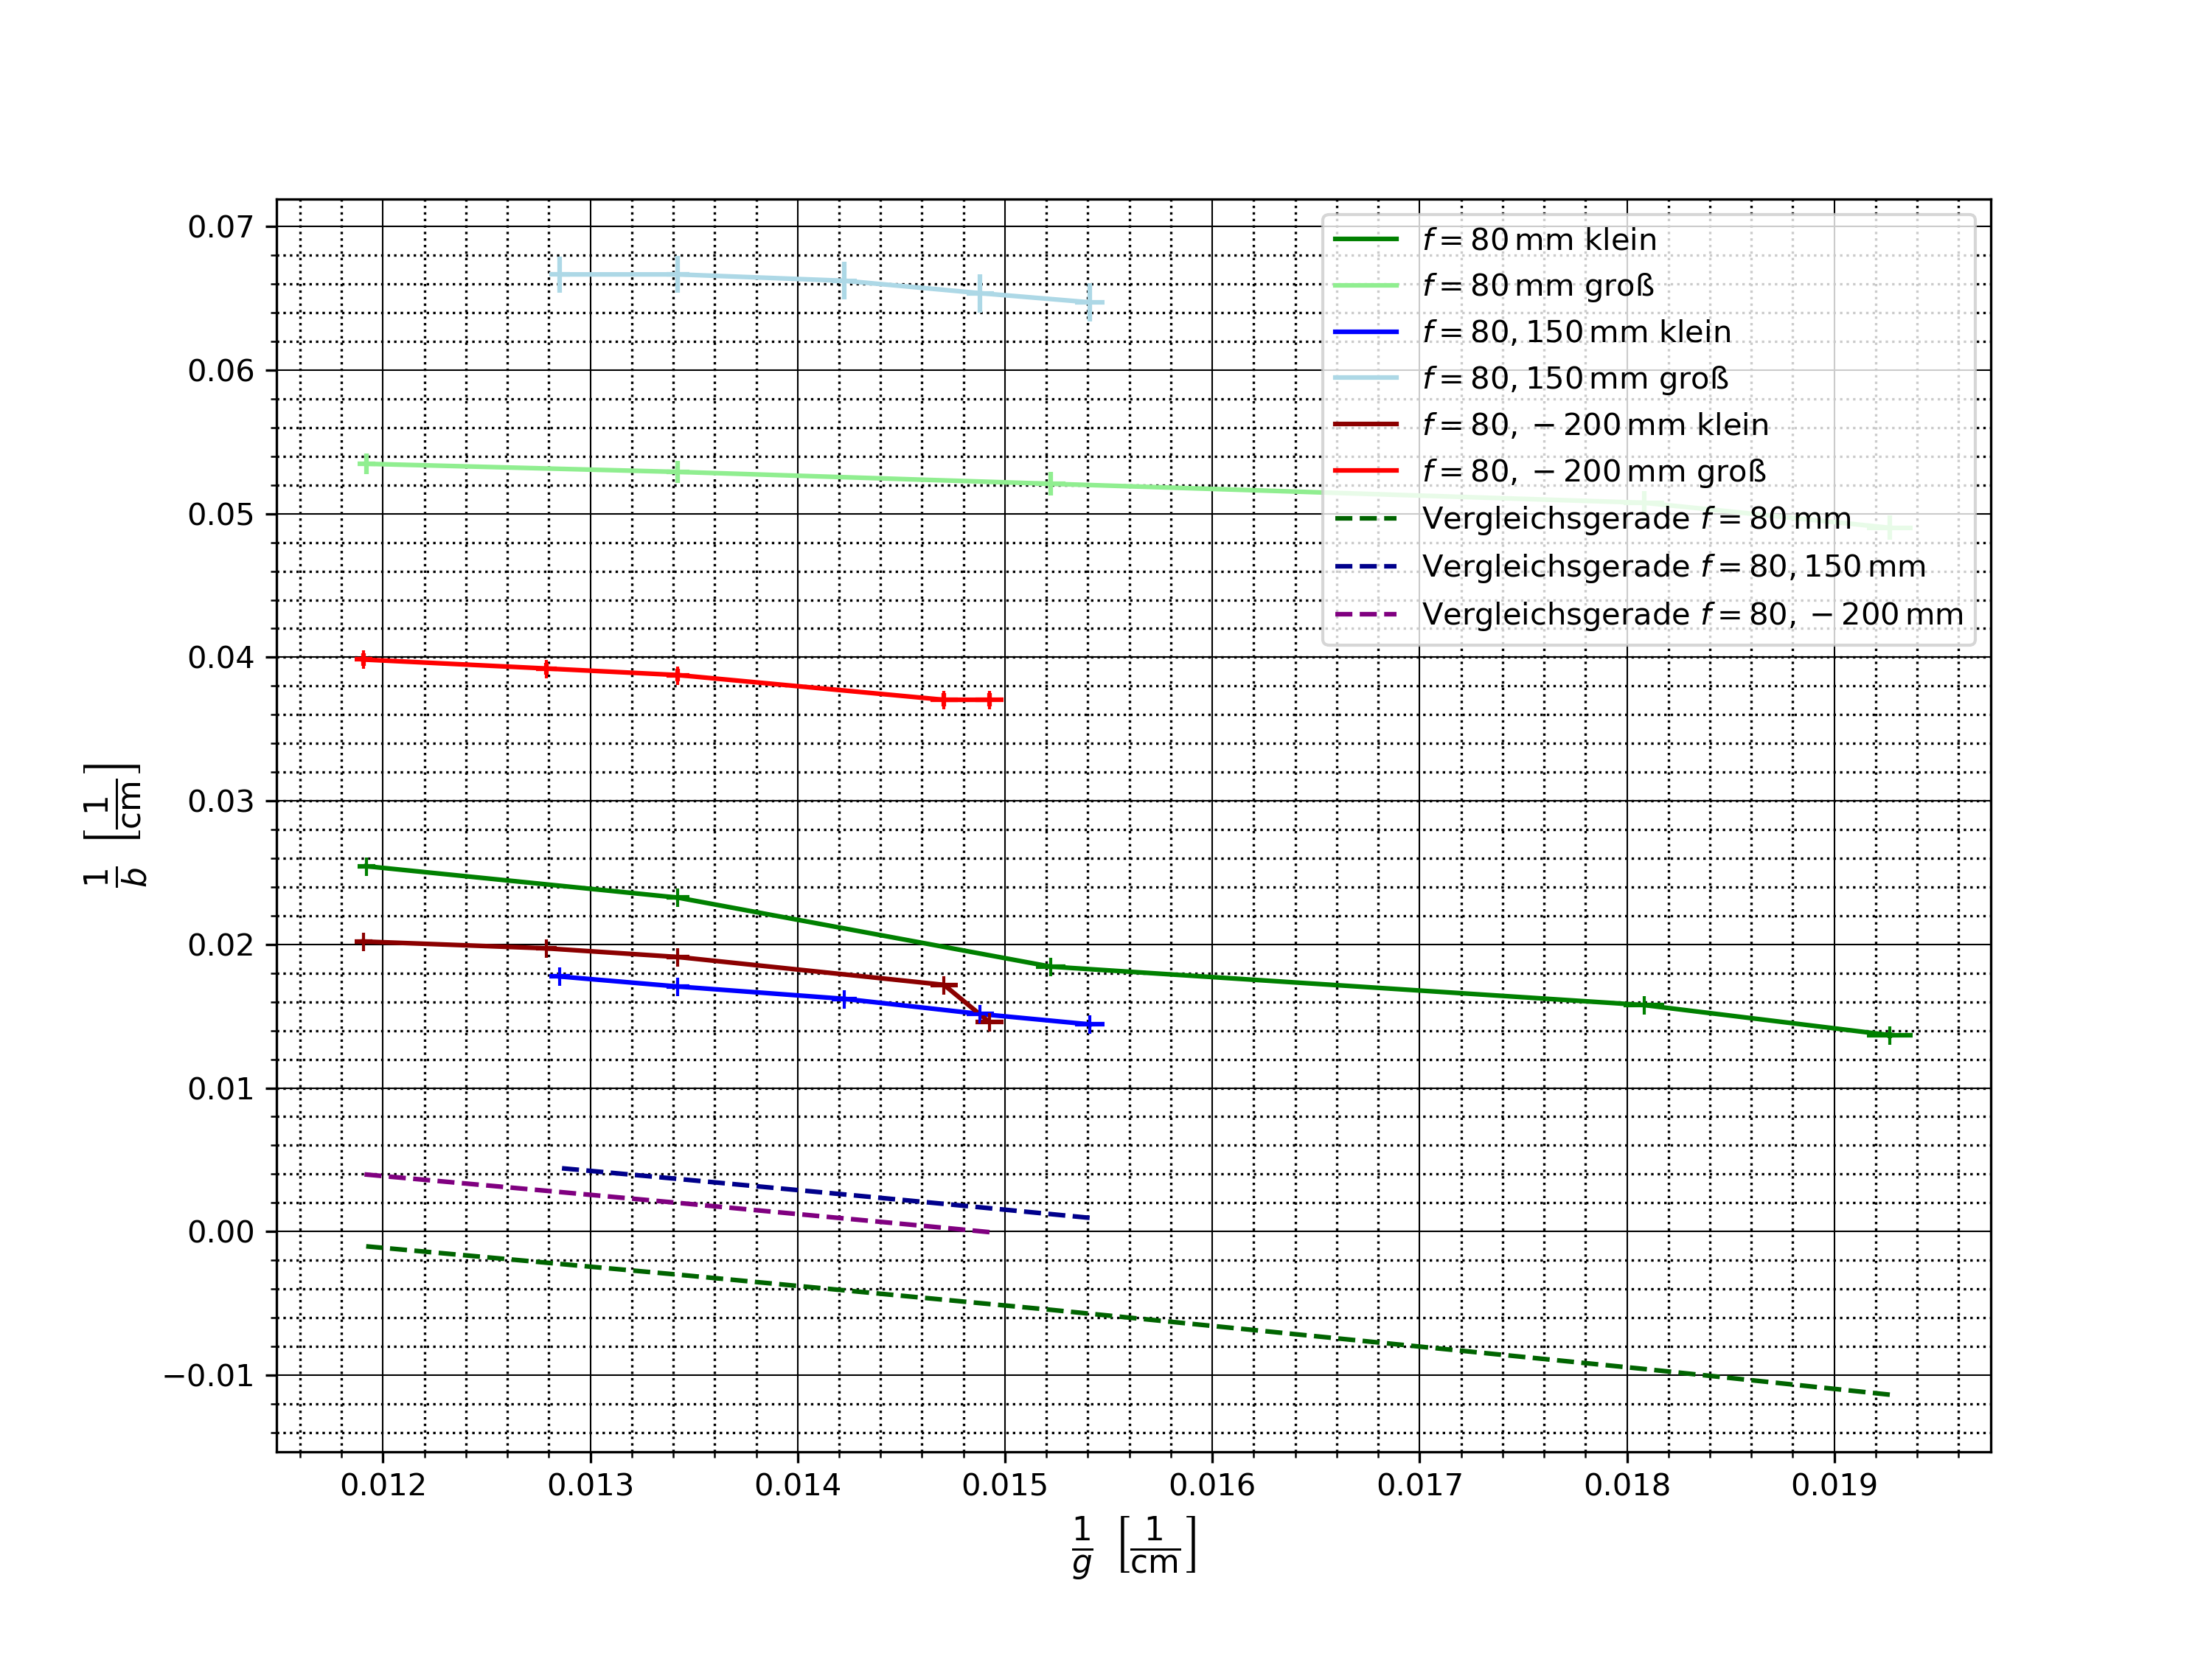
\includegraphics[width=0.8\textwidth]{part1.png}}
\renewcommand\thefigure{1}
\caption{Graphik zum ersten Teil; \nicefrac{1}{b} gegen \nicefrac{1}{g}.}
\label{Abb:1}
\end{figure}

\begin{figure}[b]
\centering
\fbox{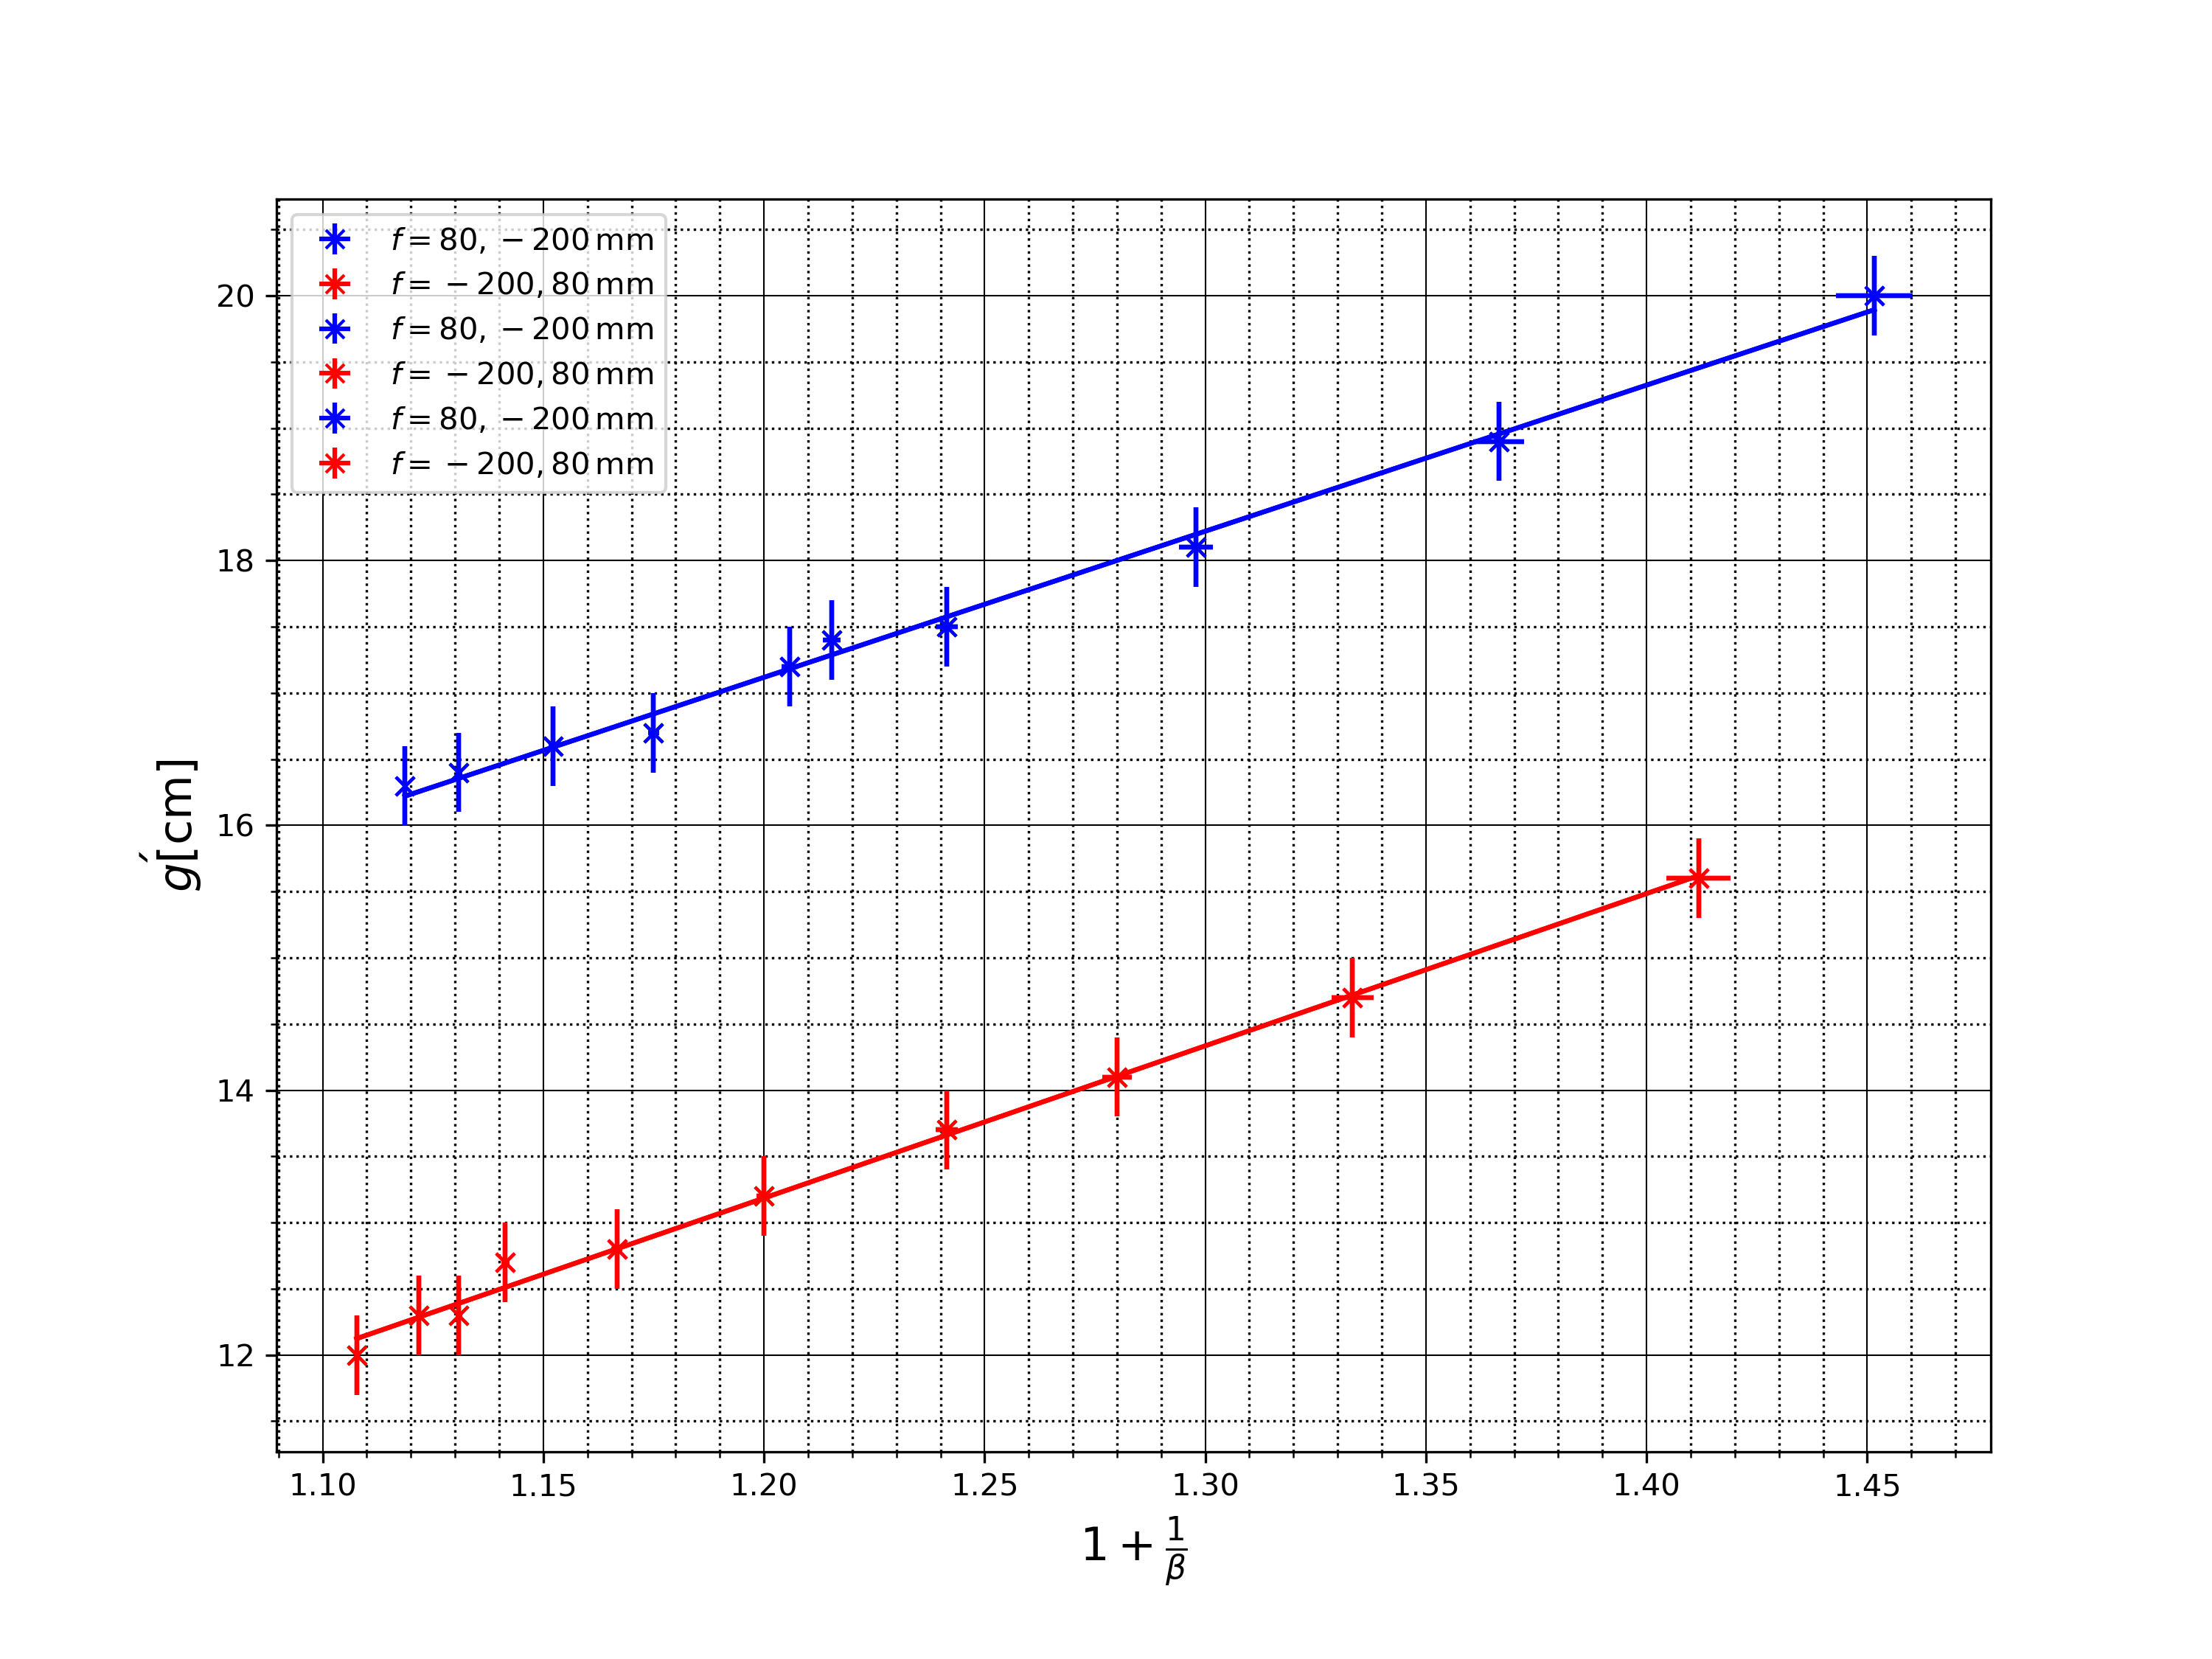
\includegraphics[width=0.8\textwidth]{g.png}}
\renewcommand\thefigure{2}
\caption[$1+\nicefrac{1}{\beta}$ gegen $g'$ dargestellt]{$1+\nicefrac{1}{\beta}$ gegen $g'$ dargestellt}
\label{Abb:g}
\end{figure}

\begin{figure}[b]
\centering
\fbox{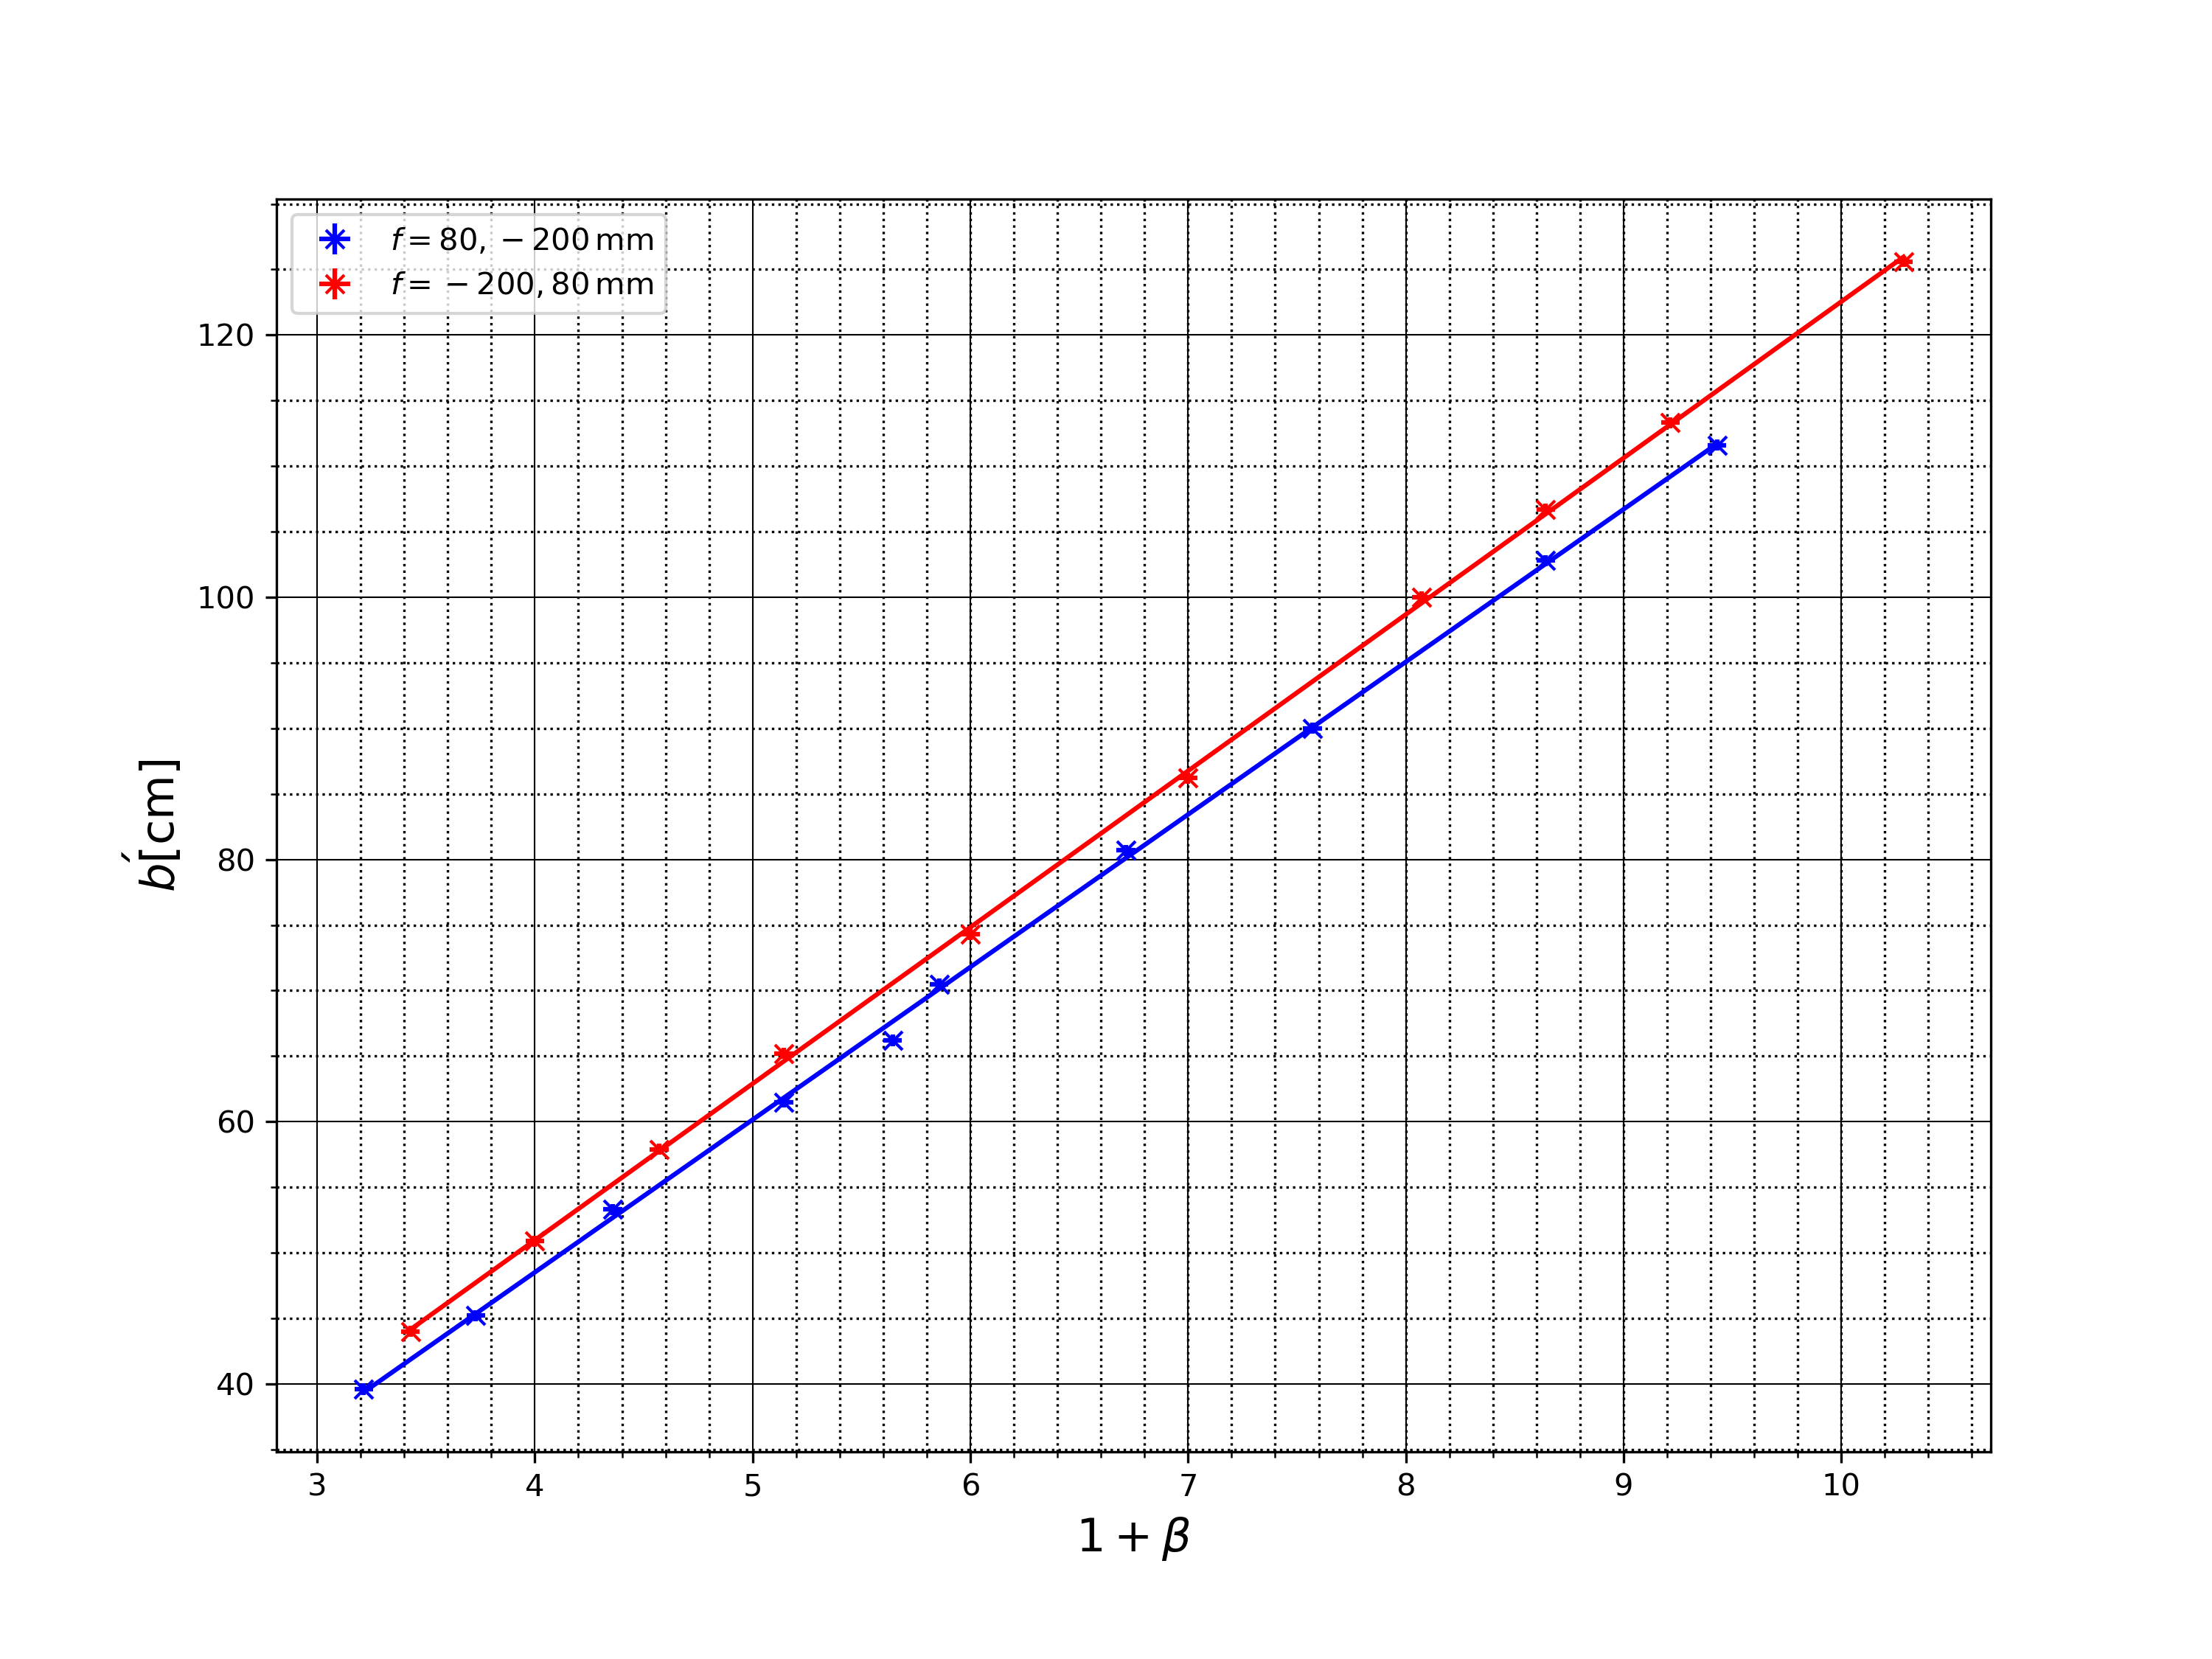
\includegraphics[width=0.8\textwidth]{b.png}}
\renewcommand\thefigure{3}
\caption[$1+{\beta}$ gegen $b'$ dargestellt]{$1+\beta$ gegen $b'$ dargestellt}
\label{Abb:b}
\end{figure}

\begin{figure}
\begin{center}
\renewcommand\thefigure{4}
\begin{tikzpicture}[scale=0.6]%, inner sep=0]
\def\sx{0.3}

% Optische Achse
\draw[dashed, thick] (-30*\sx,0) -- (50*\sx,0);
% Koordinaten Nullpunkt
\draw (0,-0.2) -- (0,0.2);

% Konkave Linse
\def\xconv{0.5} % x-Koordinate
\draw[thick, fill=yellow!30] 
     ([shift=(190:16cm)]16.5+\xconv,0) arc (190:170:16cm)
     -- ([shift=(10:16cm)] -16.5+\xconv,0)
     arc (10:-10:16cm) 
     -- ([shift=(190:16cm)]16.5+\xconv,0);

% Konvexe Linse
\def\xconx{-1.5} % x-Koordinate
\draw[thick, fill=yellow!30] ([shift=(-15:10cm)]-9+\xconx,0) arc (-15:15:10cm)
 --([shift=(165:10cm)]10+\xconx,0) arc (165:195:10cm)
 --([shift=(-15:10cm)]-9+\xconx,0);

% Gegenstand (Pfeil)
\def\Gx{-20.0*\sx}
\def\Gy{0.7}
\node [inner sep=0] (G) at (\Gx,\Gy) {};
\draw[->, ultra thick, left] (\Gx,0) to node {\tiny $7\,$mm} (G);%
\node (labG) at (\Gx,\Gy+0.5) {$G$};
% Bild (arrow)
\def\Bx{39.6*\sx}
\def\By{-1.55}
\node[inner sep=0] (B) at (\Bx,\By) {};
\draw[->, ultra thick, right] (\Bx,0) to node {\tiny $17\,$mm}  (B);
\node (labB) at (\Bx,\By-0.5) {$B$};

% Hauptebenen
\def\Hx{-3.9*\sx}
\def\Hxii{2.0*\sx}
\draw (\Hx,-4) -- (\Hx,4); % H1
\node (labH1) at (\Hx,4.5) {$H_1$};
\draw (\Hxii,-4) -- (\Hxii,4); % H2
\node (labH2) at (\Hxii,4.5) {$H_2$};

% Strahlen
% FokusG
\fill[blue] (\Hx,\By) circle [radius=0.1];
\fill[blue] (\Hxii,\By) circle [radius=0.1];
\fill[blue] (\Hx,0) circle [radius=0.1];
\fill[blue] (\Hx,\Gy) circle [radius=0.1];
\fill[blue] (\Hxii,\Gy) circle [radius=0.1];
\fill[blue] (\Hxii,0) circle [radius=0.1];
\draw[thick, color=blue] (G) -- (\Hx,\By);
\draw[thick, color=blue] (B) -- (\Hx,\By);
% FokusB
\draw[thick, color=blue] (G) -- (\Hxii,\Gy);
\draw[thick, color=blue] (B) -- (\Hxii,\Gy);
%Central
\draw[thick, color=blue] (G) -- (\Hx,0) -- (\Hxii,0)  -- (B);
               
% Label
%Fokus Punkte
\def\fxi{-11*\sx+\Hx}
\def\fxii{11.6*\sx+\Hxii}
\draw[red] (\fxi,-0.4) -- (\fxi,0.4);
\draw[red] (\fxii,-0.4) -- (\fxii,0.4);
\fill[red] (\fxi,0) circle [radius=0.1];
\fill[red] (\fxii,0) circle [radius=0.1];
\node (F1) at (\fxi,-0.8) {$F_1$};
\node (F2) at (\fxii,0.8) {$F_2$};
% Distanzen
\node (f1) at (\fxi,-3.5) {} ;
\node (h1) at (\Hx,-3.5) {} ;
\node (f2) at (\fxii,-3.5) {} ;
\node (h2) at (\Hxii,-3.5) {} ;
\draw[<->, below] (f1) to node {\tiny $f_1=11\,$cm} (h1) ;
\draw[<->, below] (f2) to node {\tiny $f_2=11.6\,$cm} (h2) ;
\draw[<->, below]%, inner sep=10] 
(h1) to node {\tiny $5.9\,$cm} (h2);

\node (g) at (\Gx,3.5) {} ;
\node (gh1) at (\Hx,3.5) {} ;
\node (b) at (\Bx,3.5) {} ;
\node (bh2) at (\Hxii,3.5) {} ;
\draw[<->, above] (g) to node {\small $g=20\,$cm} (gh1) ;
\draw[<->, above] (b) to node {\small $b=39.6\,$cm} (bh2) ;

% Koordinaten Nullpunkt
% x-Achse
\def\cy{-5}
\draw[->] (-30*\sx,\cy) -- (50*\sx,\cy);
\draw (0,-0.2+\cy) -- (0,0.2+\cy);
\draw (10*\sx,-0.2+\cy) -- (10*\sx,0.2+\cy);
\draw (-10*\sx,-0.2+\cy) -- (-10*\sx,0.2+\cy);
\draw (20*\sx,-0.2+\cy) -- (20*\sx,0.2+\cy);
\draw (-20*\sx,-0.2+\cy) -- (-20*\sx,0.2+\cy);
\draw (30*\sx,-0.2+\cy) -- (30*\sx,0.2+\cy);
\draw (-30*\sx,-0.2+\cy) -- (-30*\sx,0.2+\cy);
\node (m30) at (-30*\sx,-1+\cy) {\tiny $-30\,\mathrm{cm}$};
\node (p30) at (30*\sx,-1+\cy) {\tiny $30\,\mathrm{cm}$};
\node (zero) at (0*\sx,-1+\cy) {\tiny $0\,\mathrm{cm}$};
\draw (40*\sx,-0.2+\cy) -- (40*\sx,0.2+\cy);
\node (p40) at (40*\sx,-1+\cy) {\tiny $40\,\mathrm{cm}$};

\node (Achse) at (28*\sx,0.5) {\small optische Achse};

% y-Achse
\draw[->] (-30*\sx,0) -- (-30*\sx,3);
\draw (-30.2*\sx,1) -- (-29.8*\sx,1);
\node (y10) at (-34*\sx,1) {\tiny $10\,\mathrm{mm}$};
\draw (-30.2*\sx,2) -- (-29.8*\sx,2);
\node (y20) at (-34*\sx,2) {\tiny $20\,\mathrm{mm}$};

% Gebogener Pfeil
%\draw[->, dashed] (9.5,18) .. controls (4,18) .. (3,11.65);
\end{tikzpicture}\label{Abb:2}
\caption[Ma\ss stabsgetrue Skizze des dritten Versuchs]{Au\ss erhalb von Linsen Ma\ss stabsgetreue Skizze des dritten Versuchs}\end{center}\end{figure}



\end{document}